\chapter{Spatio-temperal movement patterns}
% Ethan + Xander
% <-- Put the correct parts in the correct sections please! -->

To automate the workflow of creating movement visualizations between buildings, a program is created. There is a distinction between two types of visualization:
\begin{enumerate}
\item Maps
\item Bar charts
\end{enumerate}
The bar plot visualizes the movement throughout the day in 24 bars. Each bar represents the movement from a selection of buildings to another selection of buildings, over a time interval of one hour. In \autoref{barcharts}, the bar charts will be discussed in more detail. For map visualization the JavaScript Leaflet.js is used, this allows for creation of an interactive user interface with a base map from Open Street Maps and visualize the buildings and movement between them. In \autoref{maps} the map visualization will be discussed in more detail. For the bar charts the Python module matplotlib was used.

\subsection{Create movement records}
The data resulting from pre-processing contains the states of where a particular device was located during a certain time period. Implicitly this also includes information on the movement of the device. If a device is first located in building A and subsequently in building B it must have moved from building A to B. However, in order to be able to retrieve the movement patterns of devices the movement should be stored explicitly. This means that each record should store the movement of one device from one building to another building or to world. Examples of movement patterns that can be retrieved from this data are: the number of devices moving from building A to B within a given time period, and the peak in movement from building A to all other buildings. 
\\\\
To create records for each movement first the preprocessed data is ordered on mac address and start time. By doing this all the subsequent states for every device are listed directly below each other (see \autoref{figure:movementrecs}). As a movement is defined by the change of one state to another, movements records can be created from every two consecutive state records (see \autoref{figure:movementrecs}. However, not every two consecutive states represent a movement. Only when the two states concern the same device and they are at different buildings they represent a movement. This means that movement records with different mac addresses or similar building id’s are filtered out (see \autoref{figure:movementrecs}.\\

\begin{figure}[H]
\centering
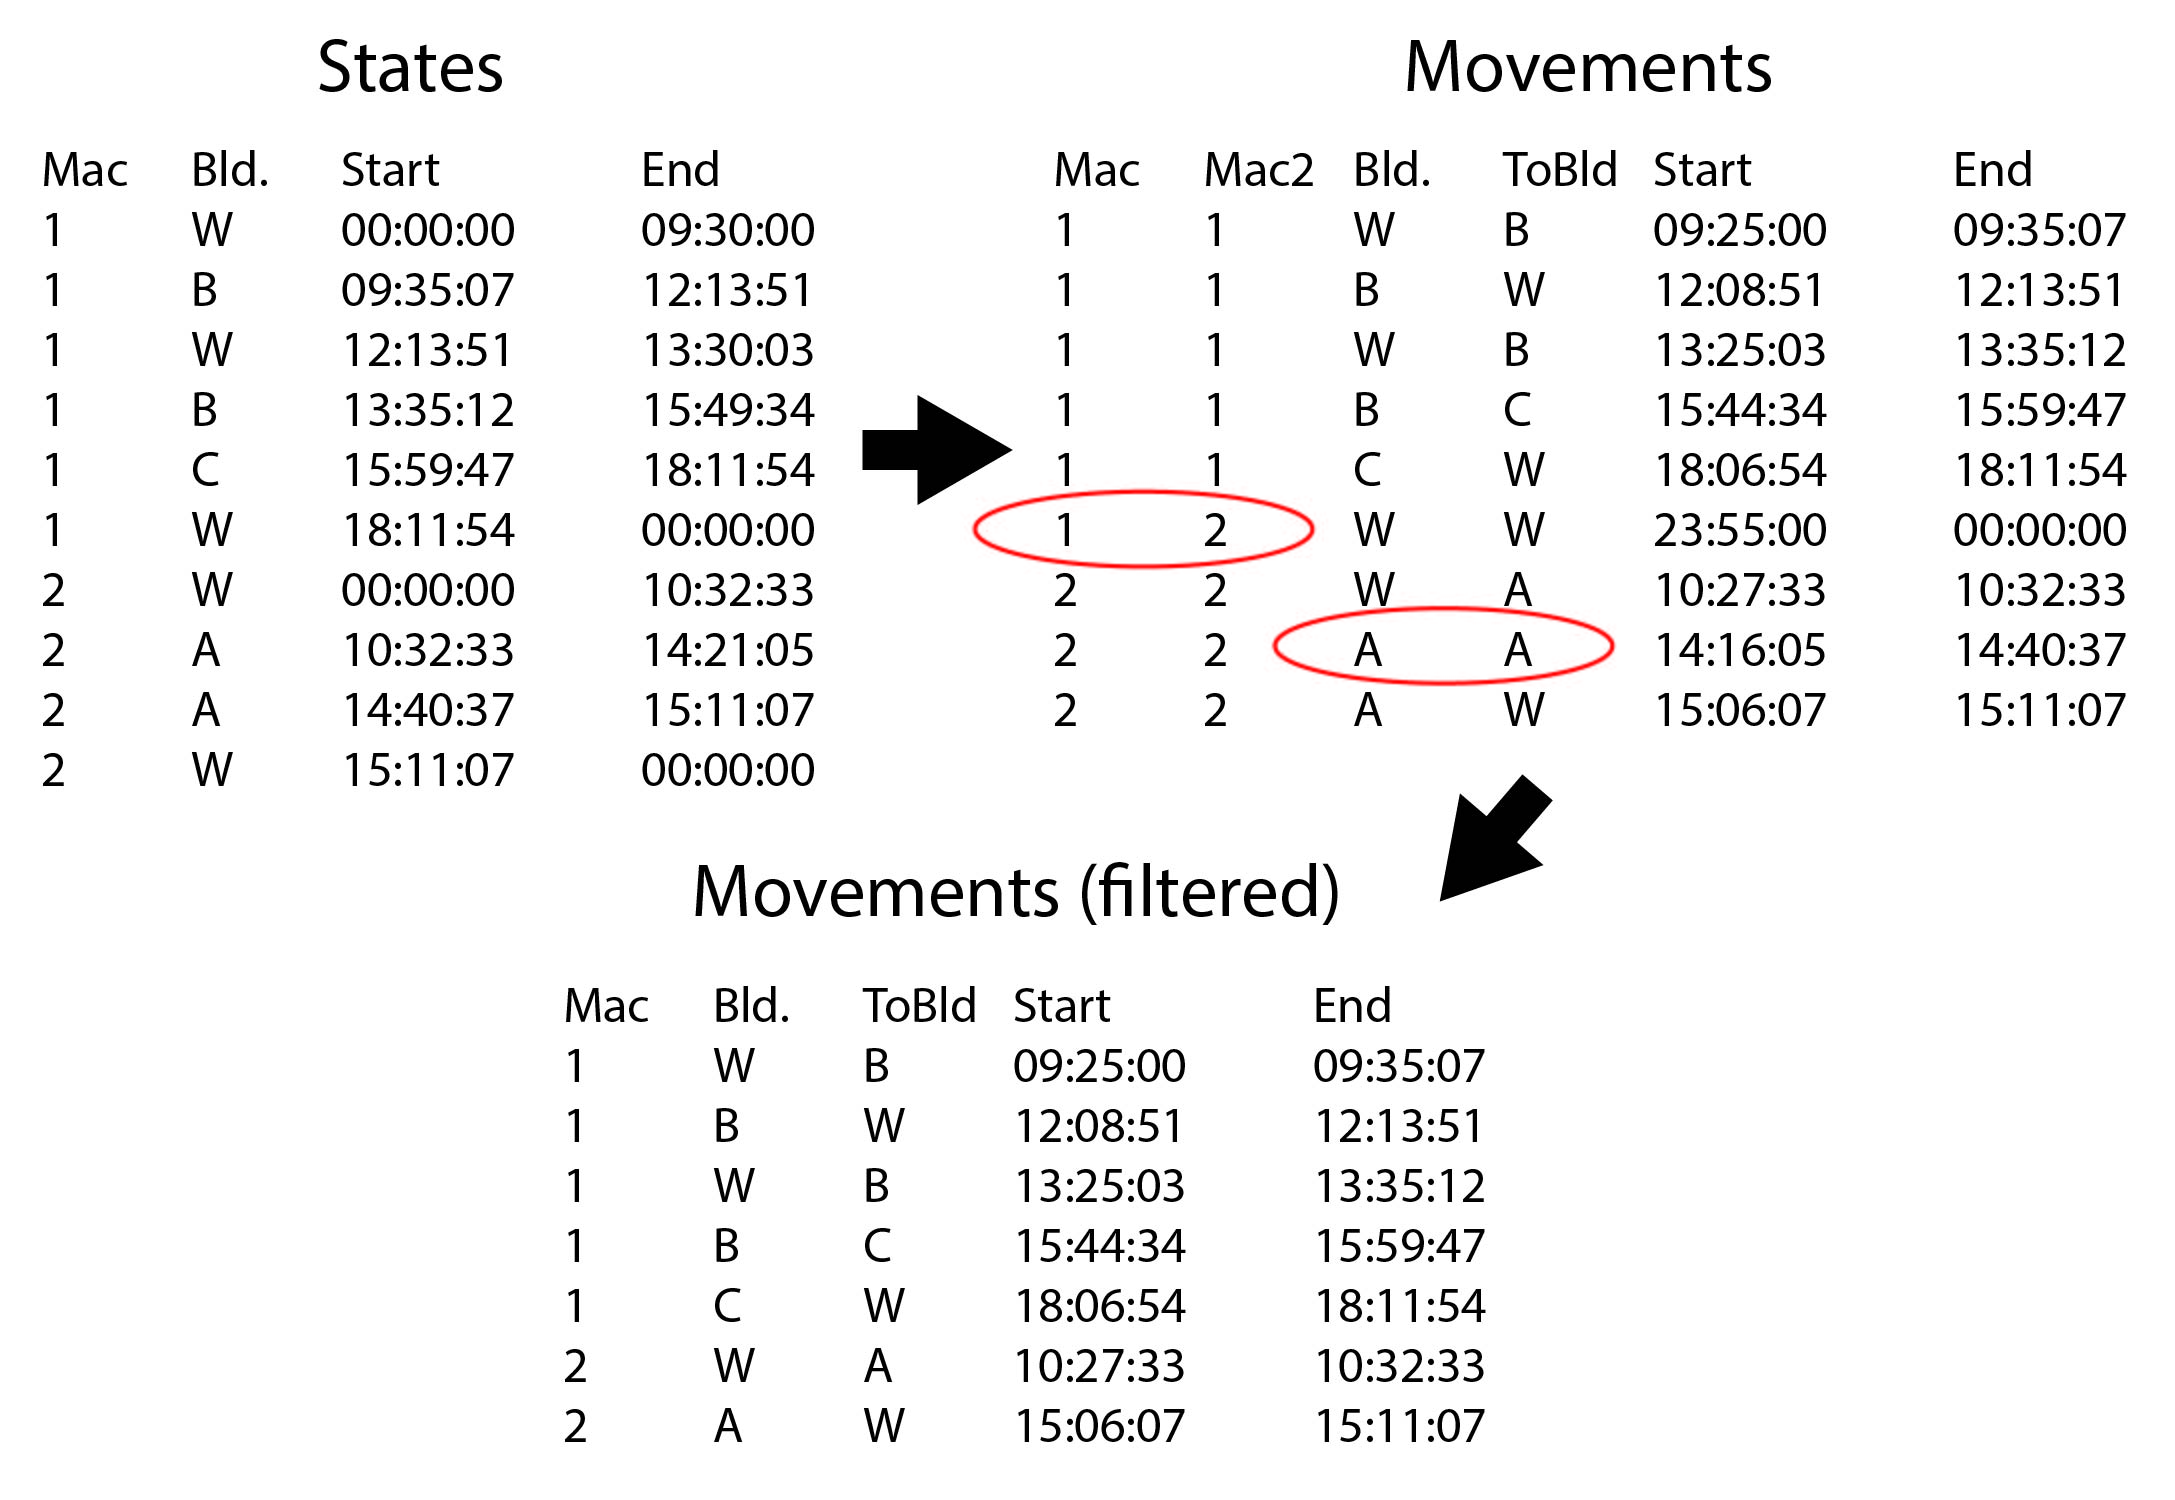
\includegraphics[scale=0.2]{movement_records.jpg}
\captionsetup{justification=centering}
\caption{Movement records}
\label{figure:movementrecs}
\end{figure}

The start and end time of the movement are defined by the end time of the previous state minus 5 minutes, and the start time of the next state (see \autoref{movement}). The reason that 5 minutes are subtracted from the end time of the previous state is that this is approximately the last moment in time the device was actually scanned at the location of the previous state. In the figure below the device is scanned 15:21 at building B. Approximately 5 minutes later (at 20:27) the device is scanned at building C. The state record of building B however continues all the way until 20:27, whilst the last time it was actually scanned at building B was 15:21. As a result it can be concluded that the movement from building B to C took place somewhere between 15:21 and 20:27. Therefore the start time of the movement between B and C can be approximated by subtracting 5 minutes from the end time of the state record at B. As can be observed in the movement from A to B is retrieved in the same way.

\begin{figure}[H]
\centering
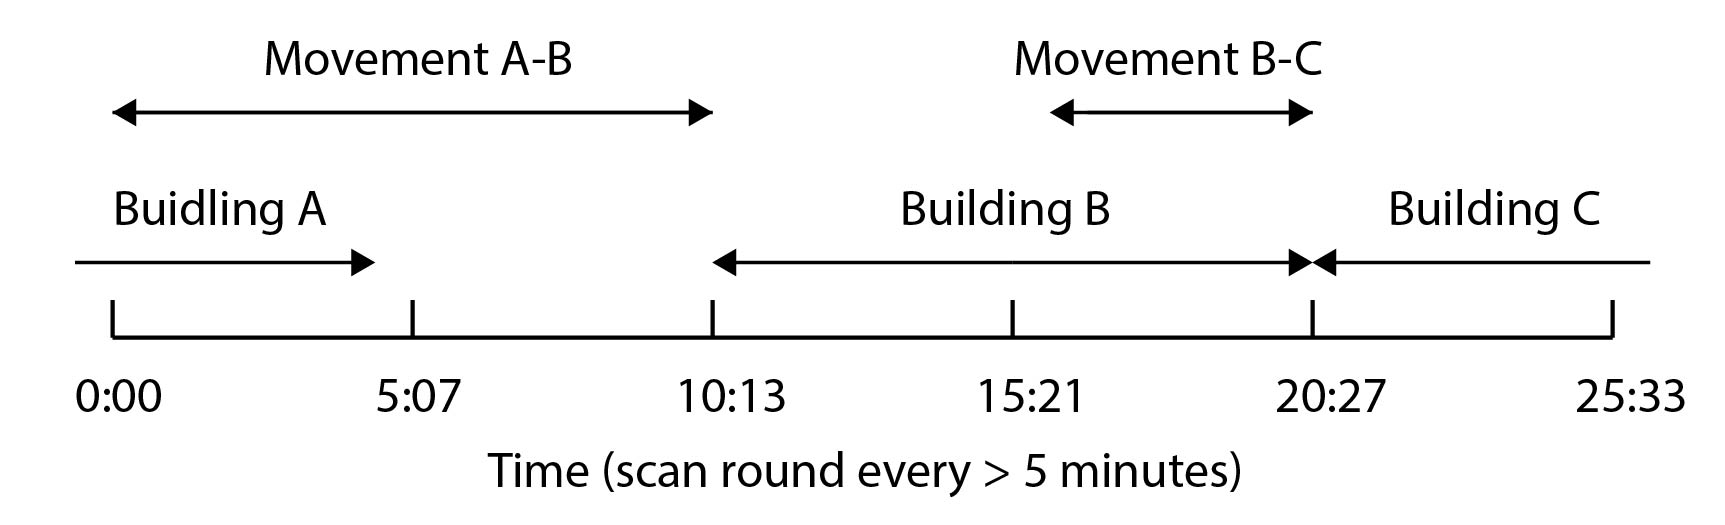
\includegraphics[scale=0.2]{movement.jpg}
\captionsetup{justification=centering}
\caption{Movement}
\label{figure:movement}
\end{figure}

\subsection{Movement over time}
As the described in section \autoref{GUI} the GUI allows a user to select particular days and specify origin and destination buildings of the movement. Based on this input the movement table can be filtered. Finally the filtered data can be visualized as the amount of movement between the specified buildings at each hour of the day. If the user has specified multiple days, the average amount of movement of these days is taken. It should be noted that the amount of movement is defined by the number of devices moving between the specified buildings. \autoref{figure:weekdays_2} gives an example of the visualization of movement over time.
\begin{figure}[H]
\centering
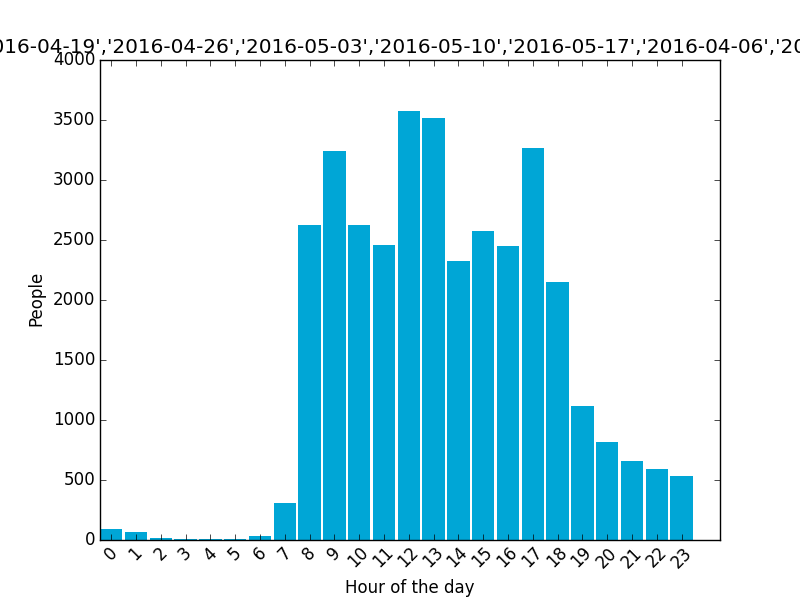
\includegraphics[scale=0.5]{12_weekdays.png}
\captionsetup{justification=centering}
\caption{Movement overtime}
\label{figure:weekdays_2}
\end{figure}

\subsection{Graphical User Interface}\label{GUI}
The Graphical User Interface (hereinafter referred to as GUI) for this work is a Python program that shows a Tkinter interface. When the user runs the program, it will display a main window, which is shown in \autoref{figure:GUImain}
\begin{figure}[H]
\centering
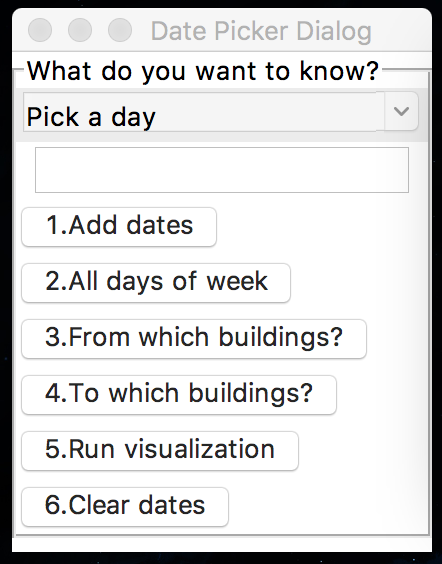
\includegraphics[scale=0.7]{GUI-main}
\captionsetup{justification=centering}
\caption{main window of GUI}
\label{figure:GUImain}
\end{figure}
\pagebreak 
To create a visualization, the user first has to select a time interval and then the buildings from and to which the movement should be visualized. The user has 2 options to select the time series for the current visualization:
\begin{enumerate}
\item Click on '1. Add dates' which will open the date picker dialog
\item Pick a day from the dropdown menu and click on '2. All days of week' 
\end{enumerate}

\begin{figure}[H]
\centering
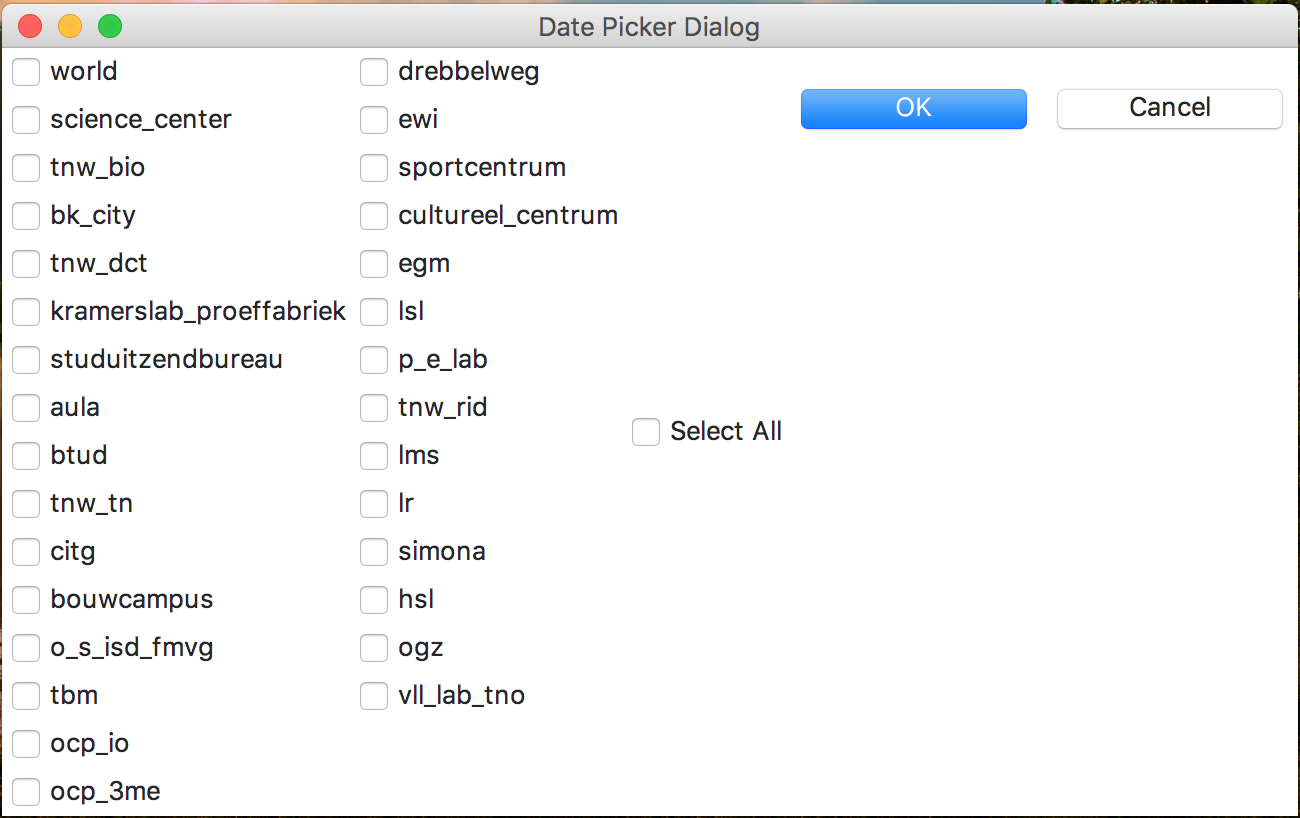
\includegraphics[scale=0.5]{GUI-buildings}
\captionsetup{justification=centering}
\caption{Buildings selection}
\label{figure:GUIbuildings}
\end{figure}

\begin{figure}[H]
\centering
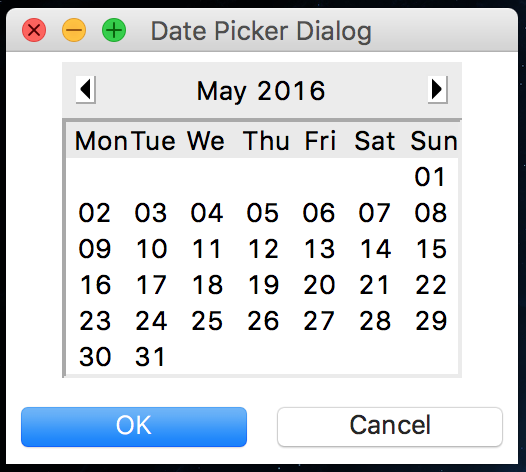
\includegraphics[scale=0.7]{GUI-dates}
\captionsetup{justification=centering}
\caption{Dates selection}
\label{figure:GUIdates}
\end{figure}

Option 1 can be used to select particular days without order. Option 2 can select 'every Tuesday' or even multiple recurring dates, such as 'every Monday to Friday'. It is also possible to combine option 1 and 2 to have for example 'every Monday and Friday the 13th of May'. 

After selecting the time series, the user has to select the buildings from and to which the movement should be visualized. The 3rd and 4th button bring up the same dialog. This dialog shows checkboxes for every building. Every building that is check will be visualized. The user also has the option to select all buildings. If the user would like to see movement from and to the same building, the user can select the same buildings twice.

\subsection{Maps}\label{maps}
In order to get an overview about how people move on the campus and further more,  find out movement patterns, a map visualization is essential. Map visualization consists of three parts: 
\begin{enumerate}
\item base map: open street map is used as a base map. There are many labels on open street map, providing more context of the environment, so it is more clear and readable compared to other base maps like satellite images.
\item building markers: building markers show the locations of the buildings. Google maps marker style is used since it is commonly used in many map application. Because the shape of the building is not useful in analyzing movement patterns between buildings, each building is regarded as a point instead of a polygon, thus a node in the network, 
\item lines: lines are the most essential part in map visualization, they represent movements between buildings.
\end{enumerate}

In the first stage of map visualization, only base map and lines are taken into consideration, building markers are not shown on the map. The line width represents the amount of movement and movements are aggregated daily regardless of the timestamp of each movement during a day. This map visualization gives an overview of the movements over a day and between which buildings there are the most movements. The following maps show the difference of the amount of movement between April 11th (weekday) and April 17th (weekend).

\begin{figure}[H]
\captionsetup[subfigure]{justification=centering}
    \centering
    \begin{subfigure}[t]{0.5\textwidth}
        \centering
        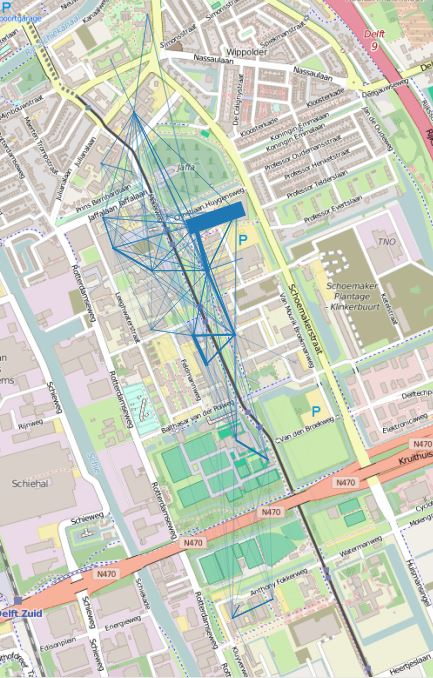
\includegraphics[scale=0.85]{pic1}
        \caption{April 11th, weekday}
    \end{subfigure}%
    ~ 
    \begin{subfigure}[t]{0.5\textwidth}
        \centering
        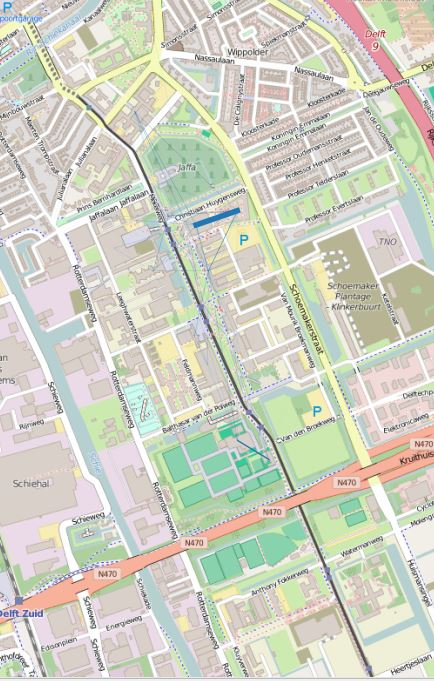
\includegraphics[scale=0.85]{pic2}
        \caption{April 17th, weekend}
    \end{subfigure}
    \captionsetup{justification=centering}
    \caption{Static visualization}
    \label{staticvisualization}
\end{figure}

It's clear that between Aula and library, there are the most movements and the amount of movements is totally different on weekday and on weekend.

Given that movements are dynamic and occuring in both space and time, a dynamic map visualization is created to display individual movement over a day with temporal information. The following screenshots of the gif file show how the movements look like at a certain time of a day:

\begin{figure}[H]
\captionsetup[subfigure]{justification=centering}
    \centering
    \begin{subfigure}[t]{0.3\textwidth}
        \centering
        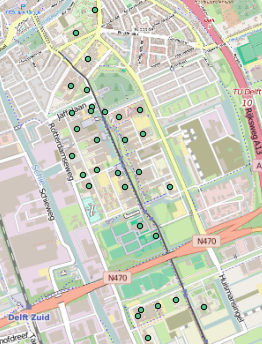
\includegraphics[scale=0.6]{frame009}
        \caption{7:00 am}
    \end{subfigure}%
    ~ 
    \begin{subfigure}[t]{0.3\textwidth}
        \centering
        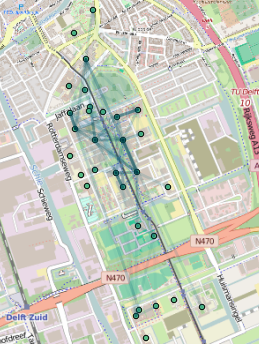
\includegraphics[scale=0.6]{frame021}
        \caption{9:00 am}
    \end{subfigure}
    \begin{subfigure}[t]{0.3\textwidth}
        \centering
        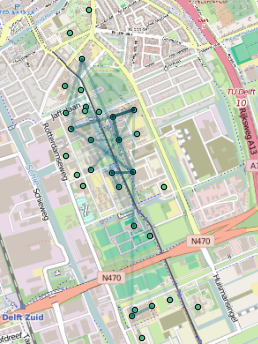
\includegraphics[scale=0.6]{frame033}
        \caption{11:00 am}
    \end{subfigure}
    \begin{subfigure}[t]{0.3\textwidth}
        \centering
        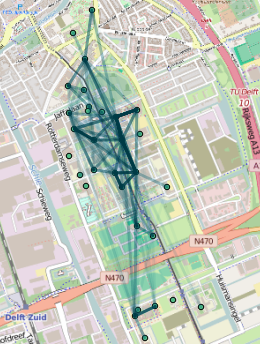
\includegraphics[scale=0.6]{frame045}
        \caption{13:00 pm}
    \end{subfigure}
    \begin{subfigure}[t]{0.3\textwidth}
        \centering
        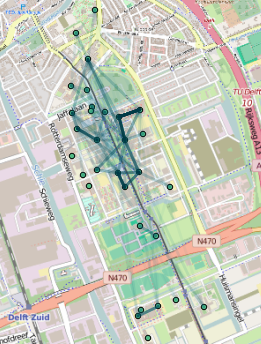
\includegraphics[scale=0.6]{frame057}
        \caption{15:00 pm}
    \end{subfigure}
    \begin{subfigure}[t]{0.3\textwidth}
        \centering
        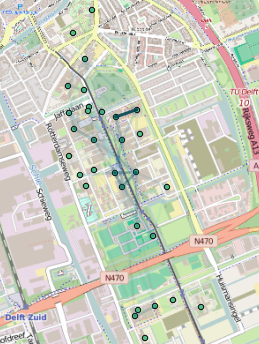
\includegraphics[scale=0.6]{frame066}
        \caption{16:30 pm}
    \end{subfigure}
    \begin{subfigure}[t]{0.3\textwidth}
        \centering
        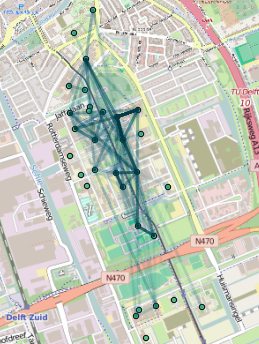
\includegraphics[scale=0.6]{frame075}
        \caption{18:00 pm}
    \end{subfigure}
    \begin{subfigure}[t]{0.3\textwidth}
        \centering
        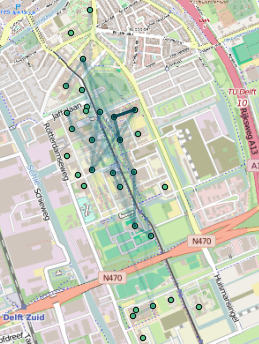
\includegraphics[scale=0.6]{frame087}
        \caption{20:00 pm}
    \end{subfigure}
    \begin{subfigure}[t]{0.3\textwidth}
        \centering
        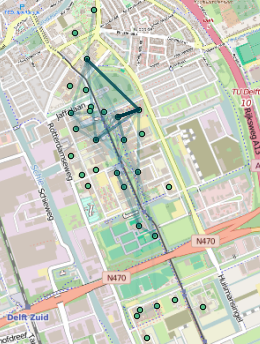
\includegraphics[scale=0.6]{frame099}
        \caption{22:00 pm}
    \end{subfigure}

    \captionsetup{justification=centering}
    \caption{Dynamic visualization of movements, April 11th}
    \label{autovisualization}
\end{figure}

In these pictures, the more movements there are, the less transparent the lines are. So generally speaking, from 7:00 am to 20:00 pm, there are two peaks at 13:00 pm and 18:00 pm. Hence, it is possible to get some insights about movement patterns from the animation. However, the dynamic map visualization doesn't provide detailed information to dig into but only an overview. So in order to find movement patterns, it is necessary to create maps containing more information, including time, direction and so forth. 

Because the amount of data is big, it is more convenient to generate maps automatically so that it will fasten the progress of finding movement patterns. According to the three components of map, there is some information needed to be collected before visualizing movement on map. The locations of buildings are collected manually on Google earth based the campus map. These locations are exported as KML file and imported into QGIS. After adding geometry columns x and y, the csv file is created and imported into database. By using $ST\_MakePoint$ function, a geometry column is created in database. In summary, the building locations are stored as the structure described in following table:

\begin{table}[H]
\centering
\begin{tabular}{|c|c|c|c|c|}
\hline 
id & name & geometry & x & y \\
\hline
0 & world & & & \\
\hline
3 & science\_ center & 010100000042A7.. & 4.36939919846287 & 52.0072322181367 \\
\hline
5 & tnw\_ bio & 010100000043AE.. & 4.37120211221402 & 52.0086132164098 \\
\hline
8 & bk\_ city & 010100000077E3.. & 4.37053698152436 & 52.0056562098059 \\
\hline
12 & tnw\_ dct & 01010000007CA.. & 4.36891378927259 & 52.0040834950037\\
\hline
.. & ... & ....& .... &....\\
\hline	
\end{tabular}
\captionsetup{justification=centering}
\caption{Building data structure}
\label{table:building}
\end{table}

There is a special 'building' called $world$ in the database. It is not an actual location, it is a virtual location which is used if someone is not scanned on the campus in a period of time. After storing the locations of buildings in the database, these locations will be extracted automatically from database to generate maps. There are two properties of lines used to deliver information:
\begin{enumerate}
\item width: line width is used to represent the amount of movements, but the amount is aggregated for both directions.
\item color: color is gradient from red to green. Red line means the movement is not symmetric that much more people move in one direction than the other, while green line means the movement is symmetric.
\end{enumerate}

Based on this map visualization, users can choose certain dates and certain buildings to generate maps automatically. It makes it easier to find out movement patterns. Since not all buildings are chosen, the map will only display the movements between several buildings, which makes the map more readable:

\begin{figure}[H]
	\centering
	\captionsetup[subfigure]{justification=centering}
	\begin{subfigure}[t]{0.48\textwidth}
	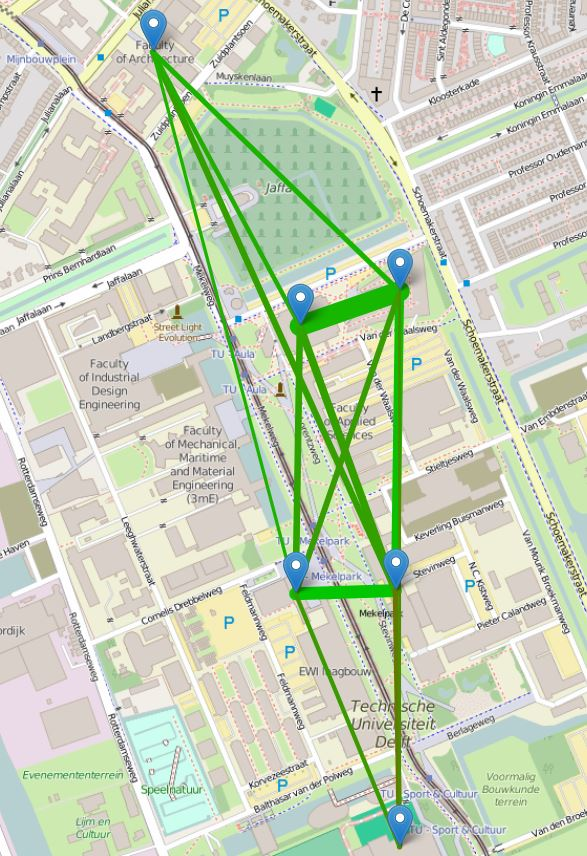
\includegraphics[scale=0.6]{pic3}
	\caption{Amount of movements on April 25th}
	\end{subfigure}
	\begin{subfigure}[t]{0.48\textwidth}
	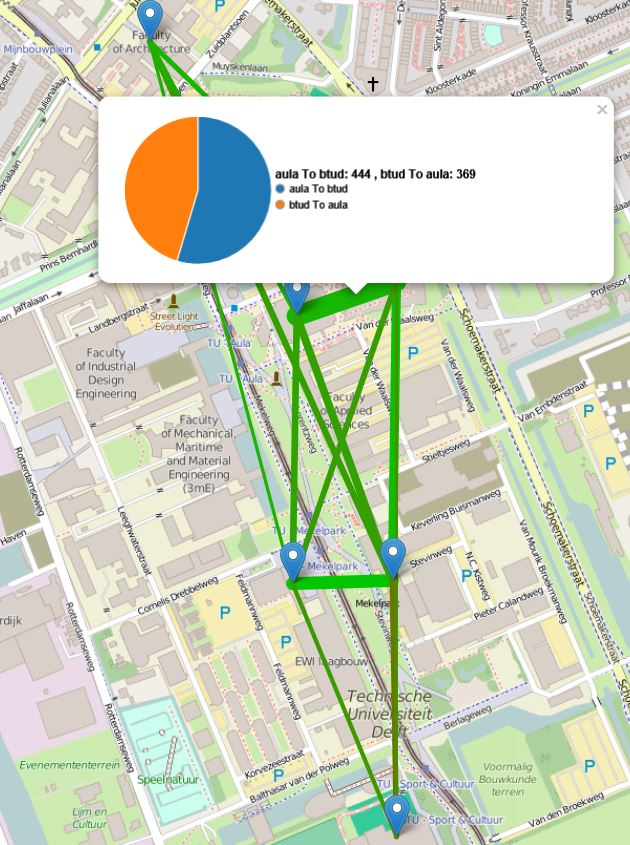
\includegraphics[scale=0.6]{pic4}
	\caption{Amount of movements in pie chart}
	\end{subfigure}
\end{figure}

As shown in the map, the lines are in different colors, which shows the symmetry of the movements. If the user is willing to know more about the movement, it is also possible to click on the line to check the amount of the movements for each direction in detail, and there will be a pie chart showing how symmetric the movements are. With the map visualization, it is easy to focus on movements which are special or interesting.

\section{Introduction}
\section{Theory / methods}
\section{Implementation}
\section{Results}\label{results}
% PLEASE UPDATE THIS PART!!! % 

The movement trajectories and the amount of movement between buildings can be visualized in maps and bar charts. The previous sections explained how the data is transformed and this section focusses on the results that can be derived from this data. Bart Valks and Iljoesja Berdrowski stated some questions that arise in their line of work and this section will try to answer these questions with the visualization in both maps and bar charts.

\subsection{Movement to the Aula on weekdays}

The department of FMRE would like to know if the faculty of Applied Sciences uses the restaurant facilities of the Aula more than other buildings, due to the fact that the two buildings are connected with a bridge on the first floor.

The graph below shows the average movement of people to the Aula on weekdays. Clearly a peak can be distinguished in the morning between 8:00 and 9:00, around lunch time and in the afternoon between 17:00 and 18:00. The morning and afternoon movements represent people moving from home to the aula and back home.
\begin{figure}[H]
\centering
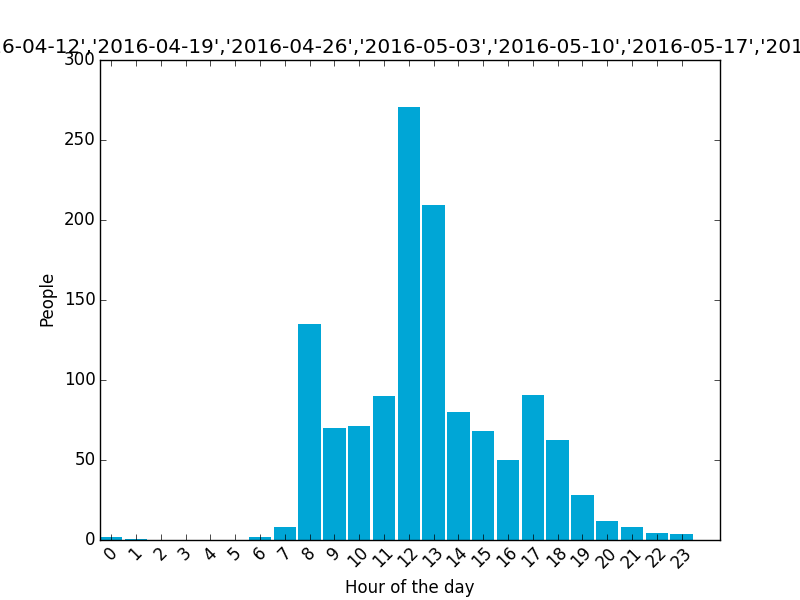
\includegraphics[scale=0.6]{all_to_aula.png}
\captionsetup{justification=centering}
\caption{All to Aula}
\label{figure:all to aula}
\end{figure}

The graph however, says nothing about which buildings contribute the most to the movement to the aula. The map image below shows the top 10 buildings with movement to the aula. It is clear that most of the movement comes from the Library. But if leaving the Library out of the equation, it is clear to conclude that the faculty of Applied Sciences uses the aula more than other faculties. The movement from TNW to the aula is 5000 people over the whole dataset, where other faculties don’t get higher amounts than 2500. 

\begin{figure}[H]
\centering
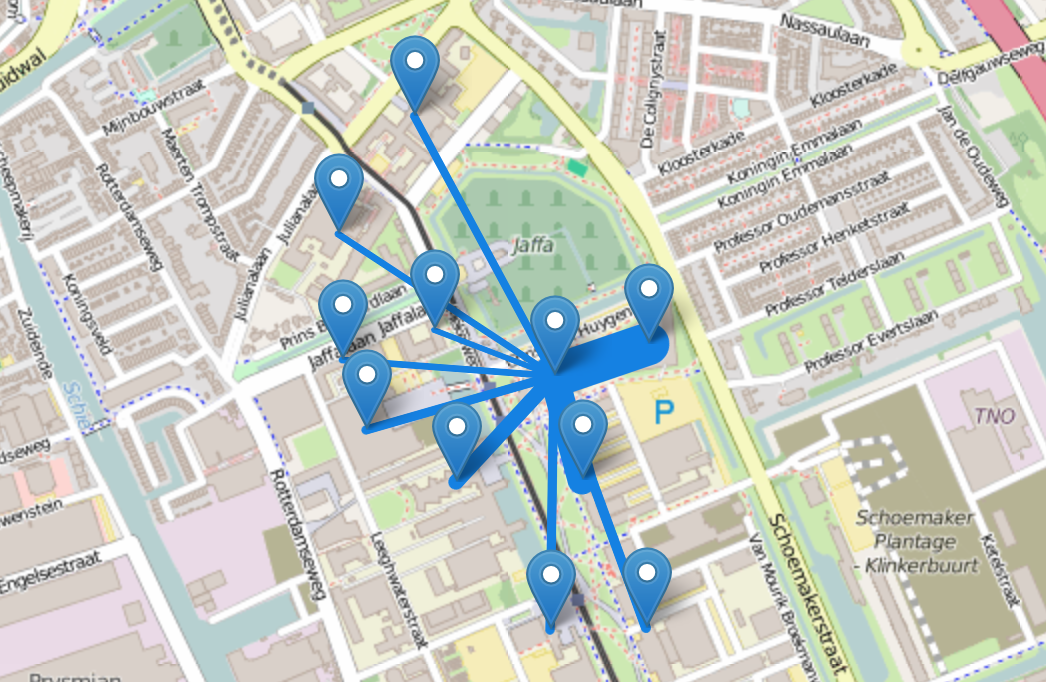
\includegraphics[scale=0.65]{map_all_to_aula.png}
\captionsetup{justification=centering}
\caption{Maps from all buildings to Aula}
\label{figure:all to aula maps}
\end{figure}

This partly confirms the assumption that FMRE made, but to be sure, the movement from the faculty of Applied Sciences must also be checked, in order to see if the movement to the aula is no exception. The result of this visualization is shown in the map image below.

\begin{figure}[H]
\centering
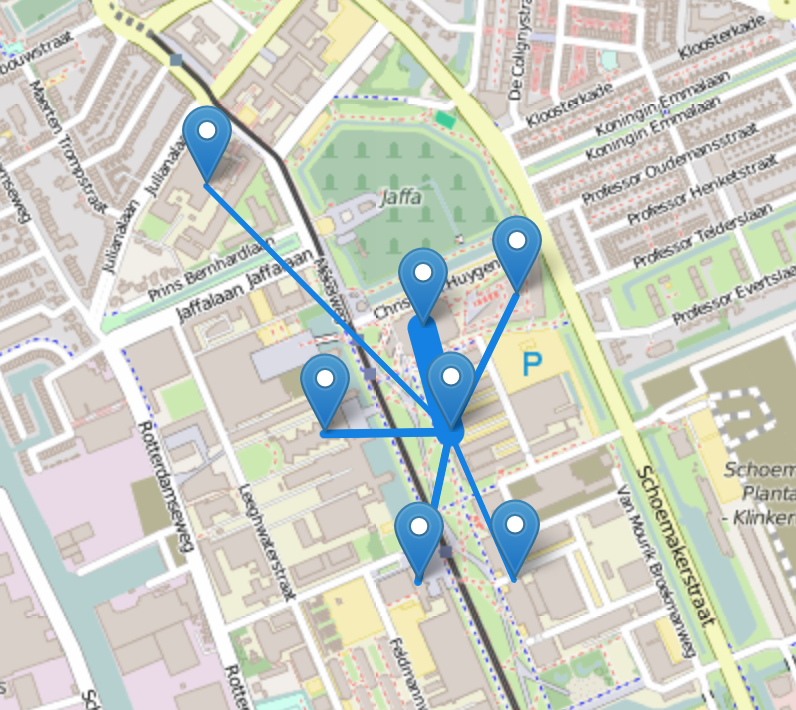
\includegraphics[scale=0.7]{map_all_to_tnw.png}
\captionsetup{justification=centering}
\caption{Maps from all buildings to TNW}
\label{figure:all to TNW maps}
\end{figure} 

This image shows that indeed most of the movement originating from the faculty of Applied Sciences is going to the Aula. The bar chart provides more insight in when this movement is taking place, which is during lunch, as expected. 
\\\\
\subsection{Movement on weekdays vs. weekends}
\begin{figure}[H]
	\centering
	\captionsetup[subfigure]{justification=centering}
	\begin{subfigure}[t]{0.48\textwidth}
	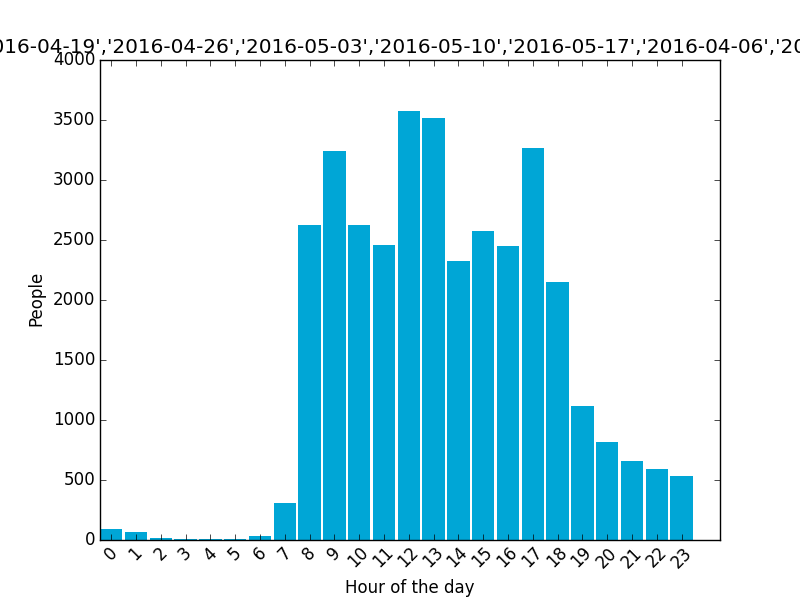
\includegraphics[scale=0.45]{12_weekdays}
	\caption{Movements on weekdays}
	\label{figure:weekdays}
	\end{subfigure}
	\begin{subfigure}[t]{0.48\textwidth}
	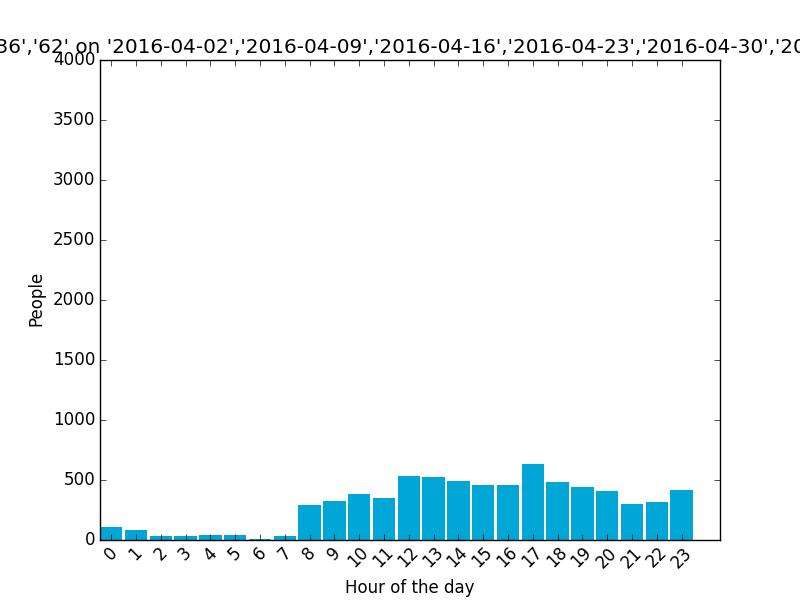
\includegraphics[scale=0.45]{12_weekends}
	\caption{Movement on weekends}
	\label{figure:weekends}
	\end{subfigure}
	\captionsetup{justification=centering}
	\caption{Bar charts of the movements}
\end{figure}

The figures above show the movement from and to the 12 most used buildings on campus. \autoref{figure:weekdays} shows the barplot for the weekdays, \autoref{figure:weekends} shows the barplot for the weekends. It is clear to see that during weekends, there is a lot less movement during weekends. Especially during lunchtime, we can see a peak during weekdays and in the morning and afternoon. In the weekend the movement to the faculties is apparently much less and more spread out over the day.\\
Interesting to see is the movement in the early morning, between 00:00 and 4:00. The library is only open from 8:00 to 2:00, but the bar chart alone does not provide enough information to draw conclusions about these movements.\\\\
\begin{figure}[H]
	\captionsetup[subfigure]{justification=centering}
	\begin{subfigure}[t]{0.48\textwidth}
	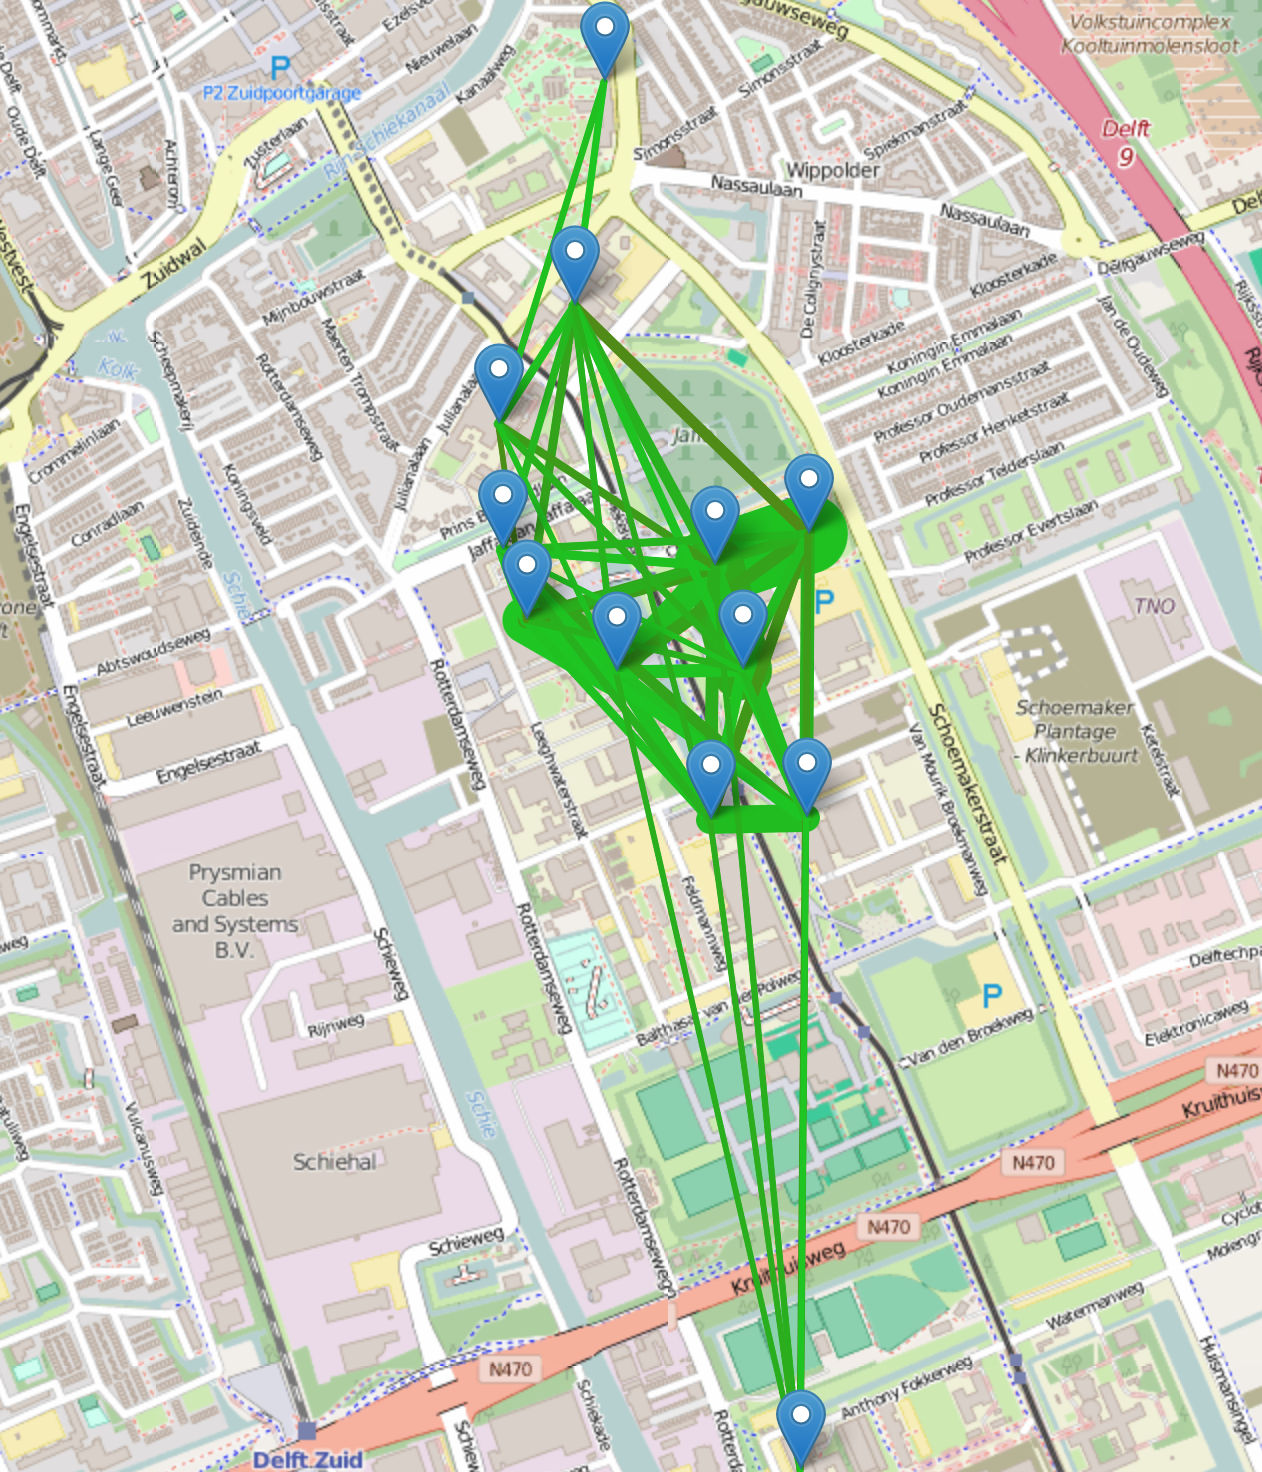
\includegraphics[scale=0.4]{12_weekdays_map}
	\caption{Movements on weekdays}
	\label{figure:map_weekdays}
	\end{subfigure}
	\begin{subfigure}[t]{0.48\textwidth}
	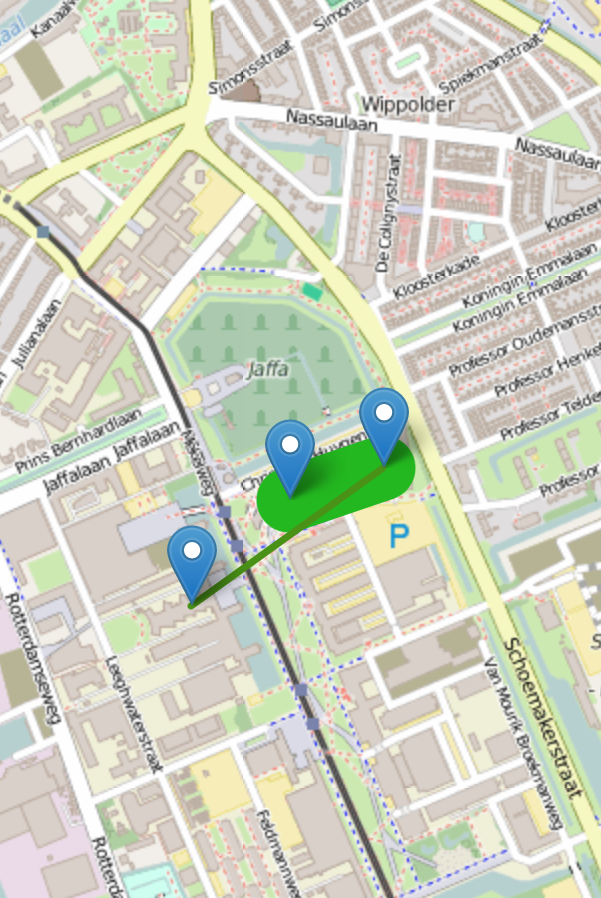
\includegraphics[scale=0.65]{12_weekends_map}
	\caption{Movements on weekends}
	\label{figure:map_weekends}
	\end{subfigure}
	\captionsetup{justification=centering}
	\caption{Maps of the movements}
\end{figure}
\autoref{figure:map_weekdays} and \autoref{figure:map_weekends} show the spread of the movement over the whole campus. Now it becomes clear that movement during weekdays is spread out over all faculties, but during weekends is only focused on the Library. There is however one exception, the faculty of 3ME. This could be explained by staff using the building with their campus card. \\

It is interesting to see that during weekdays the movement from and to a faculty is almost always symmetric, whereas in weekends this is certainly not the case. 

\subsection{Architecture as an island}
The department of FMRE also assume that architecture students and staff have the tendency to stay in their faculty and move less to other buildings on campus than other faculties. \\
Their question can be answered when looking at the movement between the faculty of architecture and all other buildings. This shows the amount of movement to other faculties, but these amounts need to be compared to the movement from other faculties (for this question IO, CiTG and LR are considered) to other buildings. \\

\begin{figure}[H]
\centering
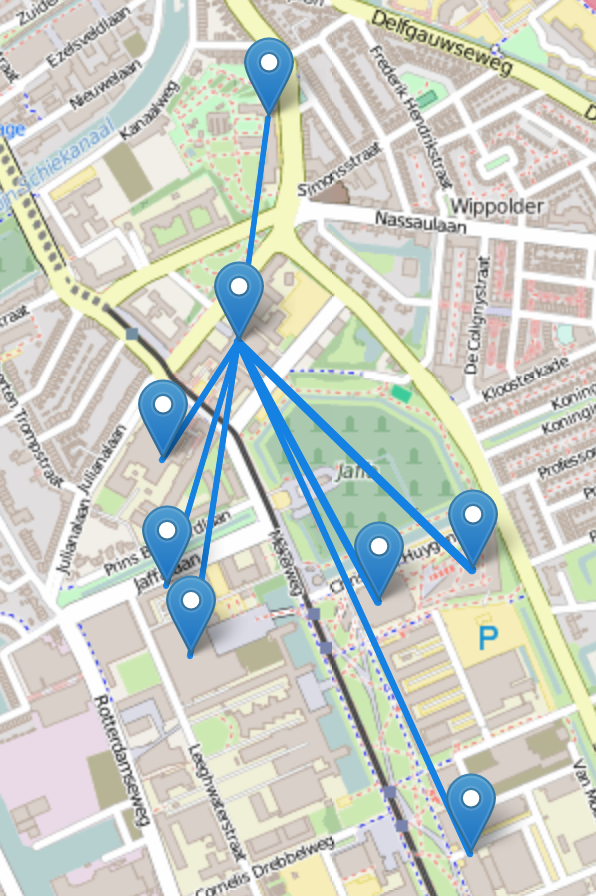
\includegraphics[scale=0.6]{bk_movement_map}
\captionsetup{justification=centering}
\caption{Movement from the faculty of Architecture}
\label{bk_map}
\end{figure} 

\autoref{bk_map} shows the movement between the faculty of architecture and other faculties. The map shows the 7 most used buildings, the movement to other faculties is only 2\% of the total movement and is left out for readability. The total amount of movement from Architecture is 4.239 people. The largest movement to any other faculty is to the Library with 1.043 people. \\

\begin{figure}[H]
\centering
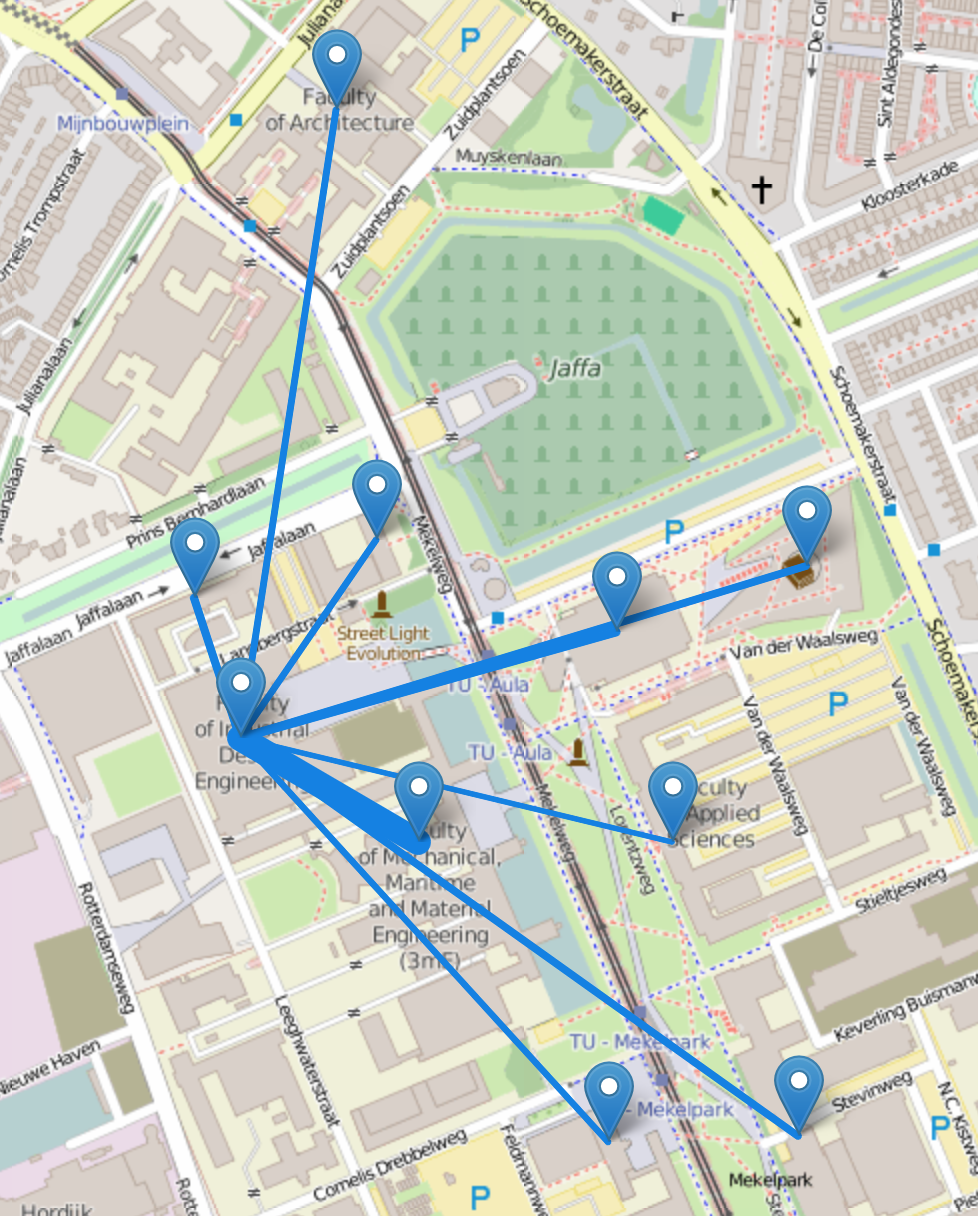
\includegraphics[scale=0.4]{IO_movement_map.png}
\captionsetup{justification=centering}
\caption{Movement from the faculty of Industrial Design}
\label{io_map}
\end{figure} 

\autoref{io_map} shows the movement from the faculty of Industrial Design to other faculties. The total amount of movement from IO is 10.933 people and the biggest movement is to the faculty of 3ME, with 4.927 people. This is already a lot more movement than the faculty of architecture.\\

\begin{figure}[H]
\centering
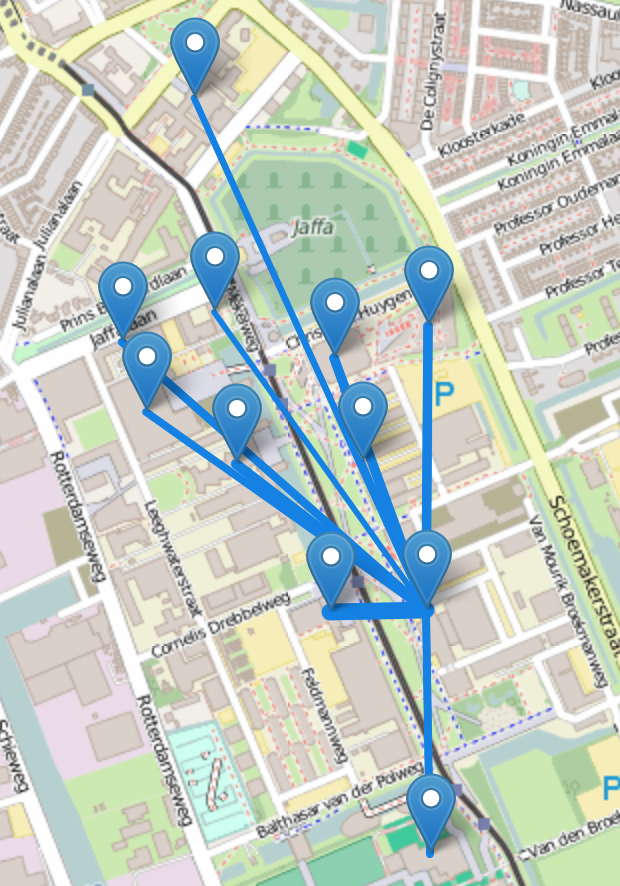
\includegraphics[scale=0.55]{citg_movement_map.png}
\captionsetup{justification=centering}
\caption{Movement from the faculty of Civil Engineering}
\label{citg_map}
\end{figure} 

\autoref{citg_map} shows the movement from the faculty of Civil Engineering to other faculties. The total amount of movement from CiTG is 11.035 people and the biggest movement is to the faculty of EWI, with 2.897 people. This is even more movement than IO.\\

\begin{figure}[H]
\centering
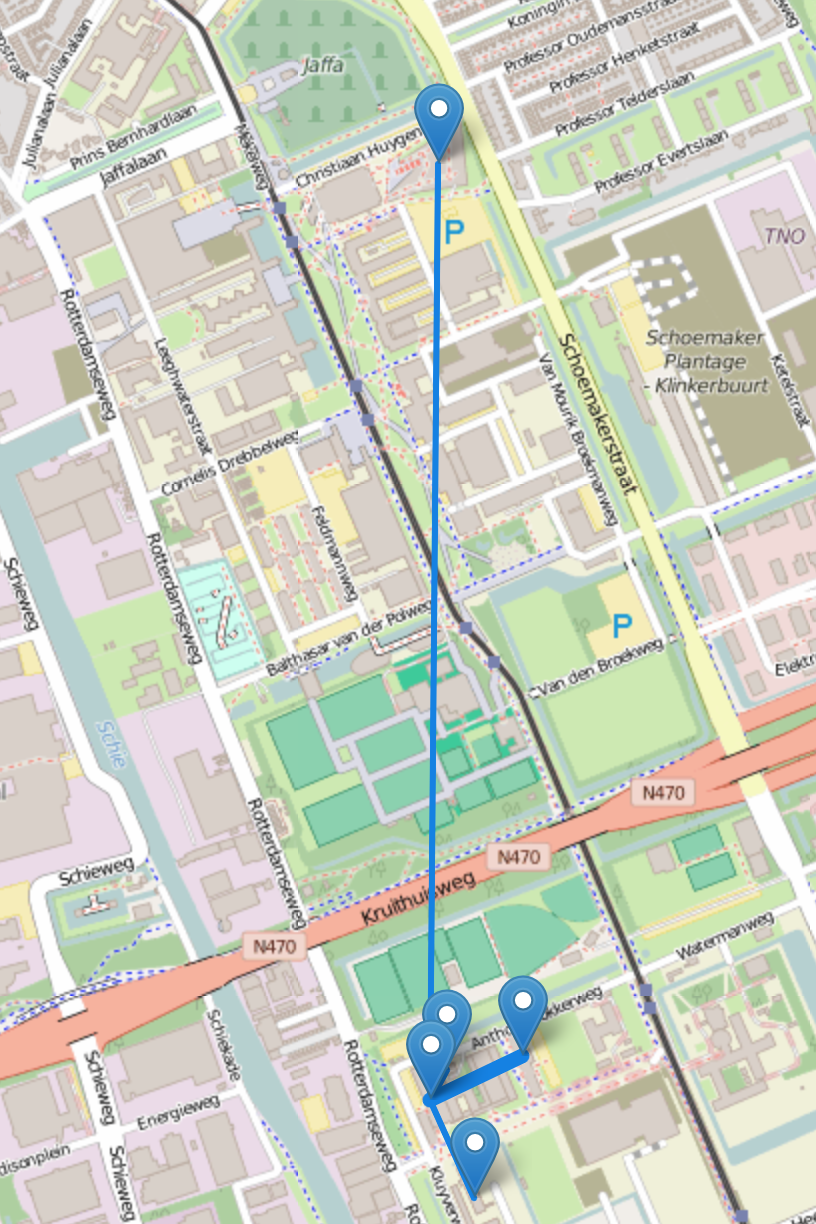
\includegraphics[scale=0.45]{lr_movement_map.png}
\captionsetup{justification=centering}
\caption{Movement from the faculty of Aerospace Engineering}
\label{lr_map}
\end{figure} 

\autoref{lr_map} shows the movement from the faculty of Aerospace Engineering to other faculties. The total amount of movement from AE is 4.348 people and the biggest movement is to the Fellowship, with 2.435 people. 

Looking at these figures we can clearly see that the movement from the faculty of architecture is much less than the movement from Civil Engineering and Industrial Design.  However, the faculty of Aerospace Engineering seems to be even more isolated than architecture. 

\subsection{Movement from and to the campus}
\begin{figure}[H]
\centering
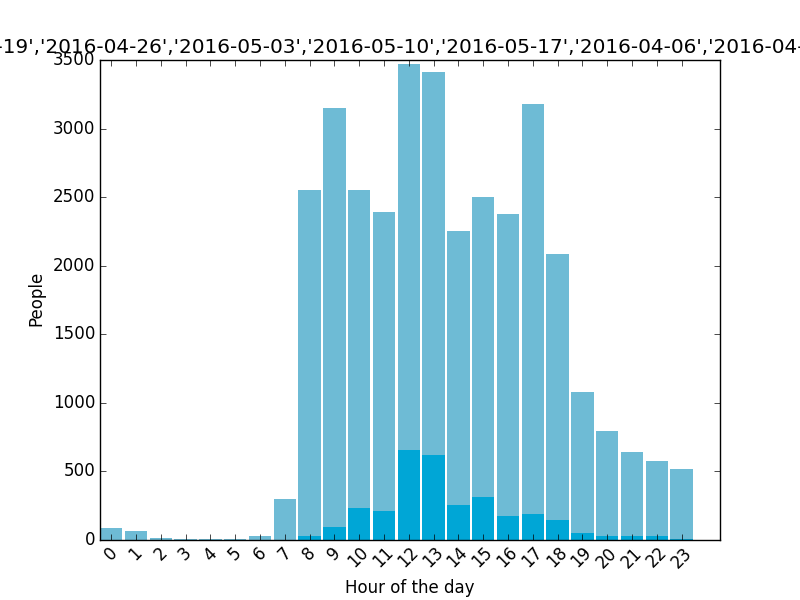
\includegraphics[scale=0.45]{weekdays.png}
\captionsetup{justification=centering}
\caption{Movement from and to the campus}
\label{newWeekdays}
\end{figure} 
The aggregated movement from the different faculties is shown in \autoref{newWeekdays}. For this bar chart, a distinction is made between movement that is either from or to the campus(in light-blue) and movement between buildings on campus (darker blue). This will result in a more accurate visualization of the data.

However, the movement from or to the campus is derived from finding gaps of more than one hour in the data, because devices going offline for more than one hour could be considered moving away from the campus. But this does also include devices that are for some reason turned off for more than one hour, such as laptops during lunch breaks or lectures. For these graphs to really accurately show the movement from and to the campus, devices should be categorized into dynamic devices, such as mobile phones and tablets, and static devices, such as laptops. That way, only the dynamic devices can be considered and the graph would be more realistic.

